\documentclass{article}

\usepackage{amsfonts}
\usepackage{amsmath,epsfig}
\usepackage{color}
\usepackage{amssymb}
\usepackage{graphicx}
\usepackage[cmtip,arrow]{xy}
\usepackage{url}
\usepackage{enumerate}
\usepackage{multirow}
\usepackage[table]{xcolor}
\usepackage{graphicx}

\begin{document}

\section{Perceptrón: XOR}
{\rowcolors{4}{blue!80!yellow!50}{blue!70!yellow!40}
\begin{tabular}{ |p{3cm}|p{3cm}|p{3cm}| }
 \hline
 \multicolumn{3}{|c|}{XOR} \\
\hline
 \multicolumn{3}{|c|}{$W(0.5, 1.5)$  $bias = 1.5$}\\
 \hline
$X_1$ & $X_2$ & $T$\\
 \hline
0 & 0 & 0 \\
0 & 1 & 1 \\
1 & 0 & 1 \\
1 & 1 & 0\\
 \hline
\end{tabular}


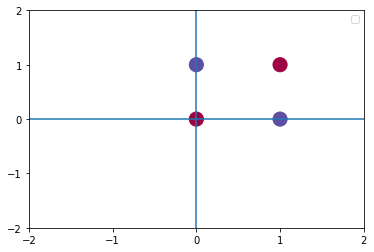
\includegraphics[scale=0.5]{xor.png}

Estos datos no son linealmente separables, por lo cual no puede aplicarse el perceptrón.
%%%%%%%%%%%%%%%%%%%%%%%%%%%%%%%%%%%%%%%%%%%%%%%%%%%%%%%%%%%%%%%%%%%%%%
\section{Perceptrón: AND}

{\rowcolors{4}{blue!80!yellow!50}{blue!70!yellow!40}
\begin{tabular}{ |p{3cm}|p{3cm}|p{3cm}| }
 \hline
 \multicolumn{3}{|c|}{And} \\
\hline
 \multicolumn{3}{|c|}{$W(0.5, 1.5)$  $bias = 1.5$}\\
 \hline
$X_1$ & $X_2$ & $T$\\
 \hline
0 & 0 & 0 \\
0 & 1 & 0 \\
1 & 0 & 0 \\
1 & 1 & 1\\
 \hline
\end{tabular}

Verficamos que sea linealmente separable:





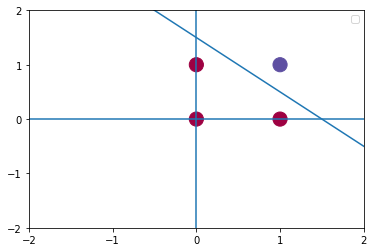
\includegraphics[scale=0.5]{descarga.png}

Se puede apreciar en la imagen que en este caso los datos son linealmente separables.
\\
\begin{itemize}
\item Época 1:
\begin{itemize}
\item Paso $1$. Entrada $P_1 = (0, 0)$, $T_1 = 0$. \\
$W(0.5, 1.5)$  $\text{bias} = 1.5$ \\

Aplicamos la regla de aprendizaje para el patrón $1$:
\begin{align*}
&\text{neta} + \text{bias}= (0 * 0.5) + (0 * 1.5) + 1.5 = 1.5\\
&a = \text{hardlim}(1.5) = 1 \\
&T_1 = 0 \neq a = 1
\end{align*}
Por lo tanto es necesario ajustar los pesos:
\begin{align*}
&e = T_1- a = 0- 1=-1, \\
&W_n = W + e* P_1 = (0.5, 1.5) + (-1) * (0,0) = (0.5, 1.5) \\
&\text{bias}_N = \text{bias} + e = 1.5 + (-1) = 0.5
\end{align*}

\item Paso $2$. Entrada $P_2 = (0, 1)$, $T_2 = 0$. \\
$W(0.5, 1.5)$  $\text{bias} = 0.5$ \\

Aplicamos la regla de aprendizaje para el patrón $2$:
\begin{align*}
&\text{neta} + \text{bias}= (0 * 0.5) + (1 * 1.5) + 0.5 = 2\\
&a = \text{hardlim}(2) = 1 \\
&T_2 = 0 \neq a = 1
\end{align*}
Por lo tanto es necesario ajustar los pesos:
\begin{align*}
&e = T_2- a = 0- 1=-1, \\
&W_n = W + e* P_2 = (0.5, 1.5) + (-1) * (0,1) = (0.5, 0.5) \\
&\text{bias}_N = \text{bias} + e = 0.5 + (-1) = -0.5
\end{align*}

\item Paso $3$. Entrada $P_3 = (1, 0)$, $T_3 = 0$. \\
$W(0.5, 0.5)$  $\text{bias} = -0.5$ \\

Aplicamos la regla de aprendizaje para el patrón $3$:
\begin{align*}
&\text{neta} + \text{bias}= (1 * 0.5) + (0 * 0.5) - 0.5 = 0\\
&a = \text{hardlim}(0) = 1 \\
&T_3 = 0 \neq a = 1
\end{align*}
Por lo tanto es necesario ajustar los pesos:
\begin{align*}
&e = T_3- a = 0- 1=-1, \\
&W_n = W + e* P_3 = (0.5, 0.5) + (-1) * (1,0) = (-0.5, 0.5) \\
&\text{bias}_N = \text{bias} + e = -0.5 + (-1) = -1.5
\end{align*}



\item Paso $4$. Entrada $P_4 = (1, 1)$, $T_4 = 1$. \\
$W(-0.5, 0.5)$  $\text{bias} = -1.5$ \\

Aplicamos la regla de aprendizaje para el patrón $4$:
\begin{align*}
&\text{neta} + \text{bias}= (1 * (-0.5)) + (1 * 0.5) - 1.5 = -1.5\\
&a = \text{hardlim}(-1.5) = 0 \\
&T_4 = 1 \neq a = 0
\end{align*}
Por lo tanto es necesario ajustar los pesos:
\begin{align*}
&e = T_4- a = 1- 0= 1, \\
&W_n = W + e* P_4 = (-0.5, 0.5) + (1) * (1,1) = (0.5, 1.5) \\
&\text{bias}_N = \text{bias} + e = -1.5 + 1 = -0.5
\end{align*}

\end{itemize}

\item Época 2:

\begin{itemize}
\item Paso $1$. Entrada $P_1 = (0, 0)$, $T_1 = 0$. \\
$W(0.5, 1.5)$  $\text{bias} = -0.5$ \\

Aplicamos la regla de aprendizaje para el patrón $1$:
\begin{align*}
&\text{neta} + \text{bias}= (0 * (0.5)) + (0 * 1.5) - 0.5 = -0.5\\
&a = \text{hardlim}(-0.5) = 0 \\
&T_1 = 0 = a = 0
\end{align*}
Por lo tanto no es necesario ajustar los pesos:

\item Paso $2$. Entrada $P_2 = (0, 1)$, $T_2 = 0$. \\
$W(0.5, 1.5)$  $\text{bias} = -0.5$ \\

Aplicamos la regla de aprendizaje para el patrón $2$:
\begin{align*}
&\text{neta} + \text{bias}= (0 * (0.5)) + (1 * 1.5) - 0.5 = 1\\
&a = \text{hardlim}(1) = 1 \\
&T_2 = 0 \neq a = 1
\end{align*}
Por lo tanto es necesario ajustar los pesos:
\begin{align*}
&e = T_2 - a = 0- 1 =  -1, \\
&W_n = W + e* P_2 = (0.5, 1.5) + (-1) * (0,1) = (0.5, 0.5) \\
&\text{bias}_N = \text{bias} + e = -0.5 - 1 = -1.5
\end{align*}

\item Paso $3$. Entrada $P_3 = (1, 0)$, $T_3 = 0$. \\
$W(0.5, 0.5)$  $\text{bias} = -1.5$ \\

Aplicamos la regla de aprendizaje para el patrón $3$:
\begin{align*}
&\text{neta} + \text{bias}= (1 * (0.5)) + (0 * 0.5) - 1.5 = -1\\
&a = \text{hardlim}(-1) = 0 \\
&T_3 = 0 = a = 0
\end{align*}
Por lo tanto no es necesario ajustar los pesos:

\item Paso $4$. Entrada $P_4 = (1, 1)$, $T_4 = 1$. \\
$W(0.5, 0.5)$  $\text{bias} = -1.5$ \\

Aplicamos la regla de aprendizaje para el patrón $4$:
\begin{align*}
&\text{neta} + \text{bias}= (1 * (0.5)) + (1 * 0.5) - 1.5 = -0.5\\
&a = \text{hardlim}(-0.5) = 0 \\
&T_4 = 1 \neq a = 0
\end{align*}
Por lo tanto es necesario ajustar los pesos:
\begin{align*}
&e = T_4 - a = 1- 0 =  1, \\
&W_n = W + e* P_4 = (0.5, 0.5) + (1) * (1,1) = (1.5, 1.5) \\
&\text{bias}_N = \text{bias} + e = -1.5 + 1 = -0.5
\end{align*}
\end{itemize}

\item Época 3:

\begin{itemize}
\item Paso $1$. Entrada $P_1 = (0, 0)$, $T_1 = 0$. \\
$W(1.5, 1.5)$  $\text{bias} = -0.5$ \\

Aplicamos la regla de aprendizaje para el patrón $1$:
\begin{align*}
&\text{neta} + \text{bias}= (0 * (1.5)) + (0 * 1.5) - 0.5 = -0.5\\
&a = \text{hardlim}(-0.5) = 0 \\
&T_1 = 0 = a = 0
\end{align*}
Por lo tanto no es necesario ajustar los pesos:

\item Paso $2$. Entrada $P_2 = (0, 1)$, $T_2 = 0$. \\
$W(1.5, 1.5)$  $\text{bias} = -0.5$ \\

Aplicamos la regla de aprendizaje para el patrón $2$:
\begin{align*}
&\text{neta} + \text{bias}= (0 * (1.5)) + (1 * 1.5) - 0.5 = 1\\
&a = \text{hardlim}(1) = 1 \\
&T_2= 0 \neq a = 1
\end{align*}
Por lo tanto es necesario ajustar los pesos:
\begin{align*}
&e = T_2 - a = 0- 1 =  -1, \\
&W_n = W + e* P_2 = (1.5, 1.5) + (-1) * (0,1) = (1.5, 0.5) \\
&\text{bias}_N = \text{bias} + e = -0.5 - 1 = -1.5
\end{align*}

\item Paso $3$. Entrada $P_3 = (1, 0)$, $T_3 = 0$. \\
$W(1.5, 0.5)$  $\text{bias} = -1.5$ \\

Aplicamos la regla de aprendizaje para el patrón $3$:
\begin{align*}
&\text{neta} + \text{bias}= (1 * (1.5)) + (0 * 0.5) - 1.5 = 0\\
&a = \text{hardlim}(0) = 1 \\
&T_3 = 0 \neq a = 1
\end{align*}
Por lo tanto es necesario ajustar los pesos:
\begin{align*}
&e = T_3 - a = 0 - 1 =  -1, \\
&W_n = W + e* P_3 = (1.5, 0.5) + (-1) * (1, 0) = (0.5, 0.5) \\
&\text{bias}_N = \text{bias} + e = -1.5 - 1 = -2.5
\end{align*}

\item Paso $4$. Entrada $P_4 = (1, 1)$, $T_4 = 1$. \\
$W(0.5, 0.5)$  $\text{bias} = -2.5$ \\

Aplicamos la regla de aprendizaje para el patrón $4$:
\begin{align*}
&\text{neta} + \text{bias}= (1 * (0.5)) + (1 * 0.5) - 2.5 = -1.5\\
&a = \text{hardlim}(-1.5) = 0 \\
&T_4 = 1 \neq a = 0
\end{align*}
Por lo tanto es necesario ajustar los pesos:
\begin{align*}
&e = T_4 - a = 1- 0 =  1, \\
&W_n = W + e* P_4 = (0.5, 0.5) + (1) * (1,1) = (1.5, 1.5) \\
&\text{bias}_N = \text{bias} + e = -2.5 + 1 = -1.5
\end{align*}
\end{itemize}

\item Época 4:
\begin{itemize}
\item Paso $1$. Entrada $P_1 = (0, 0)$, $T_1 = 0$. \\
$W(1.5, 1.5)$  $\text{bias} = -1.5$ \\

Aplicamos la regla de aprendizaje para el patrón $1$:
\begin{align*}
&\text{neta} + \text{bias}= (0 * (1.5)) + (0 * 1.5) - 1.5 = -1.5\\
&a = \text{hardlim}(-1.5) = 0 \\
&T_1 = 0 =  a = 0
\end{align*}
Por lo tanto no es necesario ajustar los pesos:

\item Paso $2$. Entrada $P_2 = (0, 1)$, $T_2 = 0$. \\
$W(1.5, 1.5)$  $\text{bias} = -1.5$ \\

Aplicamos la regla de aprendizaje para el patrón $2$:
\begin{align*}
&\text{neta} + \text{bias}= (0 * (1.5)) + (1 * 1.5) - 1.5 = 0\\
&a = \text{hardlim}(0) = 1 \\
&T_2 = 0 \neq a = 1
\end{align*}
Por lo tanto es necesario ajustar los pesos:
\begin{align*}
&e = T_2 - a = 0- 1 =  -1, \\
&W_n = W + e* P_2 = (1.5, 1.5) + (-1) * (0,1) = (1.5, 0.5) \\
&\text{bias}_N = \text{bias} + e = -1.5 - 1 = -2.5
\end{align*}

\item Paso $3$. Entrada $P_3 = (1, 0)$, $T_3 = 0$. \\
$W(1.5, 0.5)$  $\text{bias} = -2.5$ \\

Aplicamos la regla de aprendizaje para el patrón $3$:
\begin{align*}
&\text{neta} + \text{bias}= (1 * (1.5)) + (0 * 0.5) - 1.5 = -2.5\\
&a = \text{hardlim}(-2.5) = 0 \\
&T_3 = 0 = a = 0
\end{align*}
Por lo tanto no es necesario ajustar los pesos:

\item Paso $4$. Entrada $P_4 = (1, 1)$, $T_4 = 1$. \\
$W(1.5, 0.5)$  $\text{bias} = -2.5$ \\

Aplicamos la regla de aprendizaje para el patrón $4$:
\begin{align*}
&\text{neta} + \text{bias}= (1 * (1.5)) + (1 * 0.5) - 2.5 = -0.5\\
&a = \text{hardlim}(-0.5) = 0 \\
&T_4 = 1 \neq a = 0
\end{align*}
Por lo tanto es necesario ajustar los pesos:
\begin{align*}
&e = T_4 - a = 1- 0 =  1, \\
&W_n = W + e* P_4 = (1.5, 0.5) + (1) * (1,1) = (2.5, 1.5) \\
&\text{bias}_N = \text{bias} + e = -2.5 + 1 = -1.5
\end{align*}
\end{itemize}

\item Época 5:
\begin{itemize}
\item Paso $1$. Entrada $P_1 = (0, 0)$, $T_1= 0$. \\
$W(2.5, 1.5)$  $\text{bias} = -1.5$ \\

Aplicamos la regla de aprendizaje para el patrón $1$:
\begin{align*}
&\text{neta} + \text{bias}= (0 * (2.5)) + (0 * 1.5) - 1.5 = -1.5\\
&a = \text{hardlim}(-1.5) = 0 \\
&T_1 = 0 = a = 0
\end{align*}
Por lo tanto no es necesario ajustar los pesos:


\item Paso $2$. Entrada $P_2 = (0, 1)$, $T_2 = 0$. \\
$W(2.5, 1.5)$  $\text{bias} = -1.5$ \\

Aplicamos la regla de aprendizaje para el patrón $2$:
\begin{align*}
&\text{neta} + \text{bias}= (0 * (2.5)) + (1 * 1.5) - 1.5 = 0\\
&a = \text{hardlim}(0) = 1 \\
&T_2 = 0 \neq a = 1
\end{align*}
Por lo tanto es necesario ajustar los pesos:
\begin{align*}
&e = T_2 - a = 0- 1 =  -1, \\
&W_n = W + e* P_2 = (2.5, 1.5) + (-1) * (0,1) = (2.5, 0.5) \\
&\text{bias}_N = \text{bias} + e = -1.5 - 1 = -2.5
\end{align*}

\item Paso $3$. Entrada $P_3 = (1, 0)$, $T_3 = 0$. \\
$W(2.5, 0.5)$  $\text{bias} = -2.5$ \\

Aplicamos la regla de aprendizaje para el patrón $3$:
\begin{align*}
&\text{neta} + \text{bias}= (1 * (2.5)) + (0 * 0.5) - 2.5 = 0\\
&a = \text{hardlim}(0) = 1 \\
&T_3 = 0 \neq a = 1
\end{align*}
Por lo tanto es necesario ajustar los pesos:
\begin{align*}
&e = T_3 - a = 0- 1 =  -1, \\
&W_n = W + e* P_3 = (2.5, 0.5) + (-1) * (1,0) = (1.5, 0.5) \\
&\text{bias}_N = \text{bias} + e = -2.5 - 1 = -3.5
\end{align*}

\item Paso $4$. Entrada $P_4 = (1, 1)$, $T_4 = 1$. \\
$W(1.5, 0.5)$  $\text{bias} = -3.5$ \\

Aplicamos la regla de aprendizaje para el patrón $4$:
\begin{align*}
&\text{neta} + \text{bias}= (1 * (1.5)) + (1 * 0.5) - 3.5 = -1.5\\
&a = \text{hardlim}(-1.5) = 0 \\
&T_4 = 1 \neq a = 0
\end{align*}
Por lo tanto es necesario ajustar los pesos:
\begin{align*}
&e = T_4 - a = 1- 0 =  1, \\
&W_n = W + e* P_4= (1.5, 0.5) + (1) * (1,1) = (2.5, 1.5) \\
&\text{bias}_N = \text{bias} + e = -3.5 + 1 = -2.5
\end{align*}
\end{itemize}

\item Época 6:
\begin{itemize}
\item Paso $1$. Entrada $P_1 = (0, 0)$, $T_1 = 0$. \\
$W(2.5, 1.5)$  $\text{bias} = -2.5$ \\

Aplicamos la regla de aprendizaje para el patrón $1$:
\begin{align*}
&\text{neta} + \text{bias}= (0 * (2.5)) + (0 * 1.5) - 2.5 = -2.5\\
&a = \text{hardlim}(-2.5) = 0 \\
&T_1 = 0 = a = 0
\end{align*}
Por lo tanto no es necesario ajustar los pesos:

\item Paso $2$. Entrada $P_2 = (0, 1)$, $T_2 = 0$. \\
$W(2.5, 1.5)$  $\text{bias} = -2.5$ \\

Aplicamos la regla de aprendizaje para el patrón $2$:
\begin{align*}
&\text{neta} + \text{bias}= (0 * (2.5)) + (1 * 1.5) - 2.5 = -1\\
&a = \text{hardlim}(-1) = 0 \\
&T_2 = 0 = a = 0
\end{align*}
Por lo tanto no es necesario ajustar los pesos:

\item Paso $3$. Entrada $P_3 = (1, 0)$, $T_3 = 0$. \\
$W(2.5, 1.5)$  $\text{bias} = -2.5$ \\

Aplicamos la regla de aprendizaje para el patrón $3$:
\begin{align*}
&\text{neta} + \text{bias}= (1 * (2.5)) + (0 * 1.5) - 2.5 = 0\\
&a = \text{hardlim}(0) = 1 \\
&T_3 = 0 \neq a = 1
\end{align*}
Por lo tanto es necesario ajustar los pesos:
\begin{align*}
&e = T_3 - a = 0- 1 =  -1, \\
&W_n = W + e* P_3 = (2.5, 0.5) + (-1) * (1,0) = (1.5, 0.5) \\
&\text{bias}_N = \text{bias} + e = -2.5 - 1 = -3.5
\end{align*}

\item Paso $4$. Entrada $P_4 = (1, 1)$, $T_4 = 1$. \\
$W(1.5, 0.5)$  $\text{bias} = -3.5$ \\

Aplicamos la regla de aprendizaje para el patrón $4$:
\begin{align*}
&\text{neta} + \text{bias}= (1 * (1.5)) + (1 * 0.5) - 3.5 = -1.5\\
&a = \text{hardlim}(-1.5) = 0 \\
&T_4 = 1 \neq a = 0
\end{align*}
Por lo tanto es necesario ajustar los pesos:
\begin{align*}
&e = T_4 - a = 1- 0 =  1, \\
&W_n = W + e* P_4 = (1.5, 0.5) + (1) * (1,1) = (2.5, 1.5) \\
&\text{bias}_N = \text{bias} + e = -3.5 + 1 = -2.5
\end{align*}
\end{itemize}

\item Época 7:
\begin{itemize}
\item Paso $1$. Entrada $P_1 = (0, 0)$, $T_1 = 0$. \\
$W(2.5, 1.5)$  $\text{bias} = -2.5$ \\

Aplicamos la regla de aprendizaje para el patrón $1$:
\begin{align*}
&\text{neta} + \text{bias}= (0 * (2.5)) + (0 * 1.5) - 2.5 = -2.5\\
&a = \text{hardlim}(-2.5) = 0 \\
&T_1 = 0 = a = 0
\end{align*}
Por lo tanto no es necesario ajustar los pesos:

\item Paso $2$. Entrada $P_2 = (0, 1)$, $T_2 = 0$. \\
$W(2.5, 1.5)$  $\text{bias} = -2.5$ \\

Aplicamos la regla de aprendizaje para el patrón $2$:
\begin{align*}
&\text{neta} + \text{bias}= (0 * (2.5)) + (1 * 1.5) - 2.5 = -1\\
&a = \text{hardlim}(-1) = 0 \\
&T_2 = 0 = a = 0
\end{align*}
Por lo tanto no es necesario ajustar los pesos:

\item Paso $3$. Entrada $P_3 = (1, 0)$, $T_3 = 0$. \\
$W(2.5, 1.5)$  $\text{bias} = -2.5$ \\

Aplicamos la regla de aprendizaje para el patrón $3$:
\begin{align*}
&\text{neta} + \text{bias}= (1 * (2.5)) + (0 * 1.5) - 2.5 = 0\\
&a = \text{hardlim}(0) = 1 \\
&T_3 = 0 \neq a = 1
\end{align*}
Por lo tanto es necesario ajustar los pesos:
\begin{align*}
&e = T_3 - a = 0- 1 =  -1, \\
&W_n = W + e* P_3 = (2.5, 1.5) + (-1) * (1,0) = (1.5, 1.5) \\
&\text{bias}_N = \text{bias} + e = -2.5 - 1 = -3.5
\end{align*}

\item Paso $4$. Entrada $P_4 = (1, 1)$, $T_4 = 1$. \\
$W(1.5, 1.5)$  $\text{bias} = -3.5$ \\

Aplicamos la regla de aprendizaje para el patrón $4$:
\begin{align*}
&\text{neta} + \text{bias}= (1 * (1.5)) + (1 * 1.5) - 3.5 = -0.5\\
&a = \text{hardlim}(-0.5) = 0 \\
&T_4 = 1 \neq a = 0
\end{align*}
Por lo tanto es necesario ajustar los pesos:
\begin{align*}
&e = T_4 - a = 1- 0 =  1, \\
&W_n = W + e* P_4 = (1.5, 1.5) + (1) * (1,1) = (2.5, 2.5) \\
&\text{bias}_N = \text{bias} + e = -3.5 + 1 = -2.5
\end{align*}
\end{itemize}

\item Época 8:
\begin{itemize}
\item Paso $1$. Entrada $P_1 = (0, 0)$, $T_1 = 0$. \\
$W(2.5, 2.5)$  $\text{bias} = -2.5$ \\

Aplicamos la regla de aprendizaje para el patrón $1$:
\begin{align*}
&\text{neta} + \text{bias}= (0 * (2.5)) + (0 * 2.5) - 2.5 = -2.5\\
&a = \text{hardlim}(-2.5) = 0 \\
&T_1 = 0 = a = 0
\end{align*}
Por lo tanto no es necesario ajustar los pesos:

\item Paso $2$. Entrada $P_2 = (0, 1)$, $T_2 = 0$. \\
$W(2.5, 2.5)$  $\text{bias} = -2.5$ \\

Aplicamos la regla de aprendizaje para el patrón $2$:
\begin{align*}
&\text{neta} + \text{bias}= (0 * (2.5)) + (1 * 2.5) - 2.5 =0\\
&a = \text{hardlim}(0) = 1 \\
&T_2 = 0 \neq a = 1
\end{align*}
Por lo tanto es necesario ajustar los pesos:
\begin{align*}
&e = T_2 - a = 0- 1 =  -1, \\
&W_n = W + e* P_2 = (2.5, 2.5) + (-1) * (0,1) = (2.5, 1.5) \\
&\text{bias}_N = \text{bias} + e = -2.5 - 1 = -3.5
\end{align*}

\item Paso $3$. Entrada $P_3 = ( 1, 0)$, $T_3 = 0$. \\
$W(2.5, 1.5)$  $\text{bias} = -3.5$ \\

Aplicamos la regla de aprendizaje para el patrón $3$:
\begin{align*}
&\text{neta} + \text{bias}= (1 * (2.5)) + (0 * 1.5) - 3.5 = -1\\
&a = \text{hardlim}(-1) = 0 \\
&T_3 = 0 = a = 0
\end{align*}
Por lo tanto no es necesario ajustar los pesos:

\item Paso $4$. Entrada $P_4 = (1, 1)$, $T_4 = 1$. \\
$W(2.5, 1.5)$  $\text{bias} = -3.5$ \\

Aplicamos la regla de aprendizaje para el patrón $4$:
\begin{align*}
&\text{neta} + \text{bias}= (1 * (2.5)) + (1 * 1.5) - 3.5 = 0.5\\
&a = \text{hardlim}(0.5) = 1 \\
&T_4 = 1 = a = 1
\end{align*}
Por lo tanto no es necesario ajustar los pesos:
\end{itemize}

\item Época 9:
\begin{itemize}
\item Paso $1$. Entrada $P_1 = (0, 0)$, $T_1 = 0$. \\
$W(2.5, 1.5)$  $\text{bias} = -3.5$ \\

Aplicamos la regla de aprendizaje para el patrón $1$:
\begin{align*}
&\text{neta} + \text{bias}= (0 * (2.5)) + (0 * 1.5) - 3.5 = -3.5\\
&a = \text{hardlim}(-3.5) = 0 \\
&T_1 = 0 = a = 0
\end{align*}
Por lo tanto no es necesario ajustar los pesos:

\item Paso $2$. Entrada $P_2 = (0, 1)$, $T_2 = 0$. \\
$W(2.5, 1.5)$  $\text{bias} = -3.5$ \\

Aplicamos la regla de aprendizaje para el patrón $2$:
\begin{align*}
&\text{neta} + \text{bias}= (0 * (2.5)) + (1 * 1.5) - 3.5 = -2\\
&a = \text{hardlim}(-2) = 0 \\
&T_2 = 0 = a = 0
\end{align*}
Por lo tanto no es necesario ajustar los pesos:


\item Paso $3$. Entrada $P_3 = ( 1, 0)$, $T_3 = 0$. \\
$W(2.5, 1.5)$  $\text{bias} = -3.5$ \\

Aplicamos la regla de aprendizaje para el patrón $3$:
\begin{align*}
&\text{neta} + \text{bias}= (1 * (2.5)) + (0 * 1.5) - 3.5 = -1\\
&a = \text{hardlim}(-1) = 0 \\
&T_3 = 0 = a = 0
\end{align*}
Por lo tanto no es necesario ajustar los pesos:

\item Paso $4$. Entrada $P_4 = (1, 1)$, $T_4 = 1$. \\
$W(2.5, 1.5)$  $\text{bias} = -3.5$ \\

Aplicamos la regla de aprendizaje para el patrón $4$:
\begin{align*}
&\text{neta} + \text{bias}= (1 * (2.5)) + (1 * 1.5) - 3.5 = 0.5\\
&a = \text{hardlim}(0.5) = 1 \\
&T_4 = 1 = a = 1
\end{align*}
Por lo tanto no es necesario ajustar los pesos:
\end{itemize}
\end{itemize}

\begin{itemize}
\item Fase de Verificación:

\begin{itemize}
\item Paso $1$. Entrada $P_1 = (0, 0)$, $T_1 = 0$. \\
$W(2.5, 1.5)$  $\text{bias} = -3.5$ \\

Aplicamos la regla de aprendizaje para el patrón $1$:
\begin{align*}
&\text{neta} + \text{bias}= (0 * (2.5)) + (0 * 1.5) - 3.5 = -3.5\\
&a = \text{hardlim}(-3.5) = 0 \\
&T_1 = 0 = a = 0
\end{align*}


\item Paso $2$. Entrada $P_2 = (0, 1)$, $T_2 = 0$. \\
$W(2.5, 1.5)$  $\text{bias} = -3.5$ \\

Aplicamos la regla de aprendizaje para el patrón $2$:
\begin{align*}
&\text{neta} + \text{bias}= (0 * (2.5)) + (1 * 1.5) - 3.5 = -2\\
&a = \text{hardlim}(-2) = 0 \\
&T_2 = 0 = a = 0
\end{align*}



\item Paso $3$. Entrada $P_3 = ( 1, 0)$, $T_3 = 0$. \\
$W(2.5, 1.5)$  $\text{bias} = -3.5$ \\

Aplicamos la regla de aprendizaje para el patrón $3$:
\begin{align*}
&\text{neta} + \text{bias}= (1 * (2.5)) + (0 * 1.5) - 3.5 = -1\\
&a = \text{hardlim}(-1) = 0 \\
&T_3 = 0 = a = 0
\end{align*}


\item Paso $4$. Entrada $P_4 = (1, 1)$, $T_4 = 1$. \\
$W(2.5, 1.5)$  $\text{bias} = -3.5$ \\

Aplicamos la regla de aprendizaje para el patrón $4$:
\begin{align*}
&\text{neta} + \text{bias}= (1 * (2.5)) + (1 * 1.5) - 3.5 = 0.5\\
&a = \text{hardlim}(0.5) = 1 \\
&T_4 = 1 = a = 1
\end{align*}

\end{itemize}
\end{itemize}
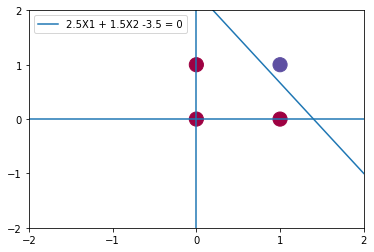
\includegraphics[scale=0.5]{descarga1.png}

Los resultados obtenidos son:
\begin{align*}
\text{Pesos: } W(2.5, 1.5) \\
\text{bias: }  -3.5
\end{align*}
\end{document}